\chapter{Испытание и обоснование эффективности предлагаемых подходов}
\section{Проектирование ПО}
Предложенные алгоритмы были реализованы с использованием языка программирования Python и сервиса построения 
маршрутов Open Source Routing Machine (OSRM) для расчёта расстояния между узлами графа по городским дорогам.
Программный код опубликован на хостинге Github (подробнее в Приложении Б).

\section{Методика проведения эксперимента}
Для оценки эффективности алгоритма и изучения его специфики, были проведены эксперименты в ходе которых 
менялось количество узлов в дорожном графе и количество создаваемых маршрутов в городской сети, а также 
несколько вариантов реализации данного метода. Наиболее интересным случаем является, когда обрабатывается 
большое число узлов в графе или большое число геопространственных данных.

% \subsection{Данные}
Были сгенерированы данных о предпочтениях по перемещению жителей среднего по размерам города с примерным 
числом жителей около 350 000. В качестве результата, было получено 6000 пар точек отправления-назначения или 
12000 точек в общей сложности. Матрица корреспонденций в данном случае имеет очень большой размер 
\( 6000 \times 6000 \) элементов, где элемент с индексом \( i, j \) имеет значение \( 0 \) -- отсутствие связи 
между \( i \)-ой и \( j \)-ой точкой, а \( 1 \) соответственно связь.

Для того, чтобы уменьшить размер матрицы корреспонденций и понять наиболее густонаселённые места, был 
применён алгоритм алгоритм кластеризации точек отправления-назначения, который не входит в рассмотрение в 
данной работе.

% \subsection{Критерии}

% \subsection{Методика}
Для получения понимания какое количество кластеров (или узлов) влияет на эффективность работы предложенного 
алгоритма было предложено произвести варьирование параметров: количество кластеров и количество маршрутов для 
построения.

\chapter{Методология и результаты}
\section{Проведение эксперимента и описание результатов}
По мере того как количество кластеров изменяется получаем различные варианты производительности алгоритма. 
В проводимых экспериментах число узлов изменяется в диапазоне от 100 до 300.

Количество маршрутов для построения так же влияет на скорость работы предложенного алгоритма. Очевидно, что 
минимальное количество маршрутов определяется числом пар терминальных маршрутов. В данном случае варьирование 
числа маршрутов было произведено в интервале от 8 до 100 в зависимости от количества узлов.

В эксперименте использовалось эмпирическое правило, что число узлов должно быть в 20 раз больше, чем число 
маршрутов. Для упрощения оценки производительности применяется общая длина сети в качестве критерия качества.
Поскольку эта оценка производится во внешнем цикле, то она не имеет большого влияния на выполнение алгоритма.
Кроме того не была использована информация о возможных пробках влияющая на процедуру выбора соответствующего 
узла.

Чтобы понять эффективность работы алгоритма в зависимости от окружающей среды, были разработаны три 
альтернативных реализации:
\begin{enumerate}
    \item Последовательная реализация (или graph) алгоритма основанного на графе дорог. В данной реализации 
        предполагается, что связь между узлами может быть проведена по прямой линии, несмотря на состояние 
        дорог. Эту реализацию можно рассматривать в качестве базовой.
    \item Последовательная реализация с использованием OSRM (или S.OSRM) -- это усовершенствованная версия 
        предыдущей стратегии, где расстояние между кластерами рассчитывается с использование движка 
        маршрутизации OSRM по дорожной сети.
    \item Параллельная версия с использованием OSRM (или P.OSRM) предполагает возможность в распараллеливании 
        внутреннего цикла алгоритма.  
\end{enumerate}

\clearpage

\subsection{Последовательная реализация}
Данная реализация является наиболее простой из всех с точки зрения расчёта расстояния. В данном случае 
применяется евклидово расстояние между узлами с использованием проекции Меркатора. Эта версия может быть 
интересна в качестве ориентира в тесте производительности.

В таблице \ref{tab:second_alg} приведены результаты для нескольких узлов (до 100) показывающие слабое влияние 
на время выполнения программы.

Рисунок \ref{fig:network-01} представляет результат работы алгоритма на 100 узлах для 8 маршрутов.

\subsection{Последовательная с использованием OSRM}
Использование OSRM является узким местом в данной реализации и решение данной задачи ускоряет время 
вычисления очень значительно, до 50 раз. Однако увеличение числа маршрутов сокращает время работы и повышает 
скорость обработки.

\subsection{Параллельная с использованием OSRM}
Для ускорения алгоритма \ref{alg:min-length} предлагается распараллеливание внутреннего цикла (шаги 4-5).
Распараллеливание можно произвести, так как обработка происходит по независимым друг от друга парам узлов 
графа. В данной реализации была испытана 8-ми поточная версия.

Рисунок \ref{fig:network-02} представляет результат работы алгоритма (последовательной или параллельной 
версии с использование OSRM) на 100 узлах для 14 маршрутов.

\subsection{Результаты}
Результаты представлены на рисунках \ref{fig:result-01} и \ref{fig:result-02}, а также в таблице 
\ref{tab:second_alg}. Рисунки представлены в логарифмической шкале по оси ординат, для более удобного 
анализа данных.

\begin{figure}[ht!]
    \centering
    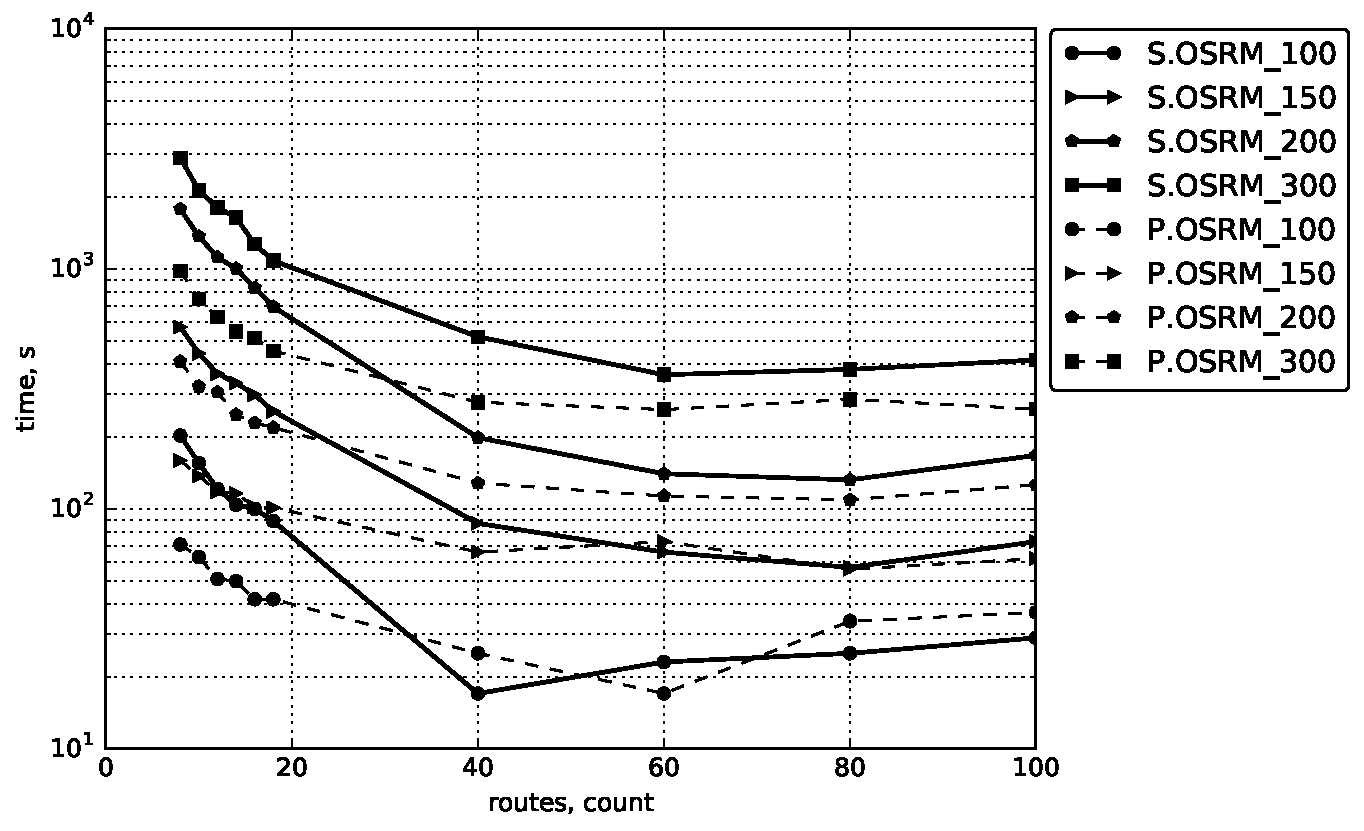
\includegraphics[width=\textwidth]{result-01}
    \caption{Зависимость времени построения от количества маршрутов}
    \label{fig:result-01}
\end{figure}

\begin{figure}[ht!]
    \centering
    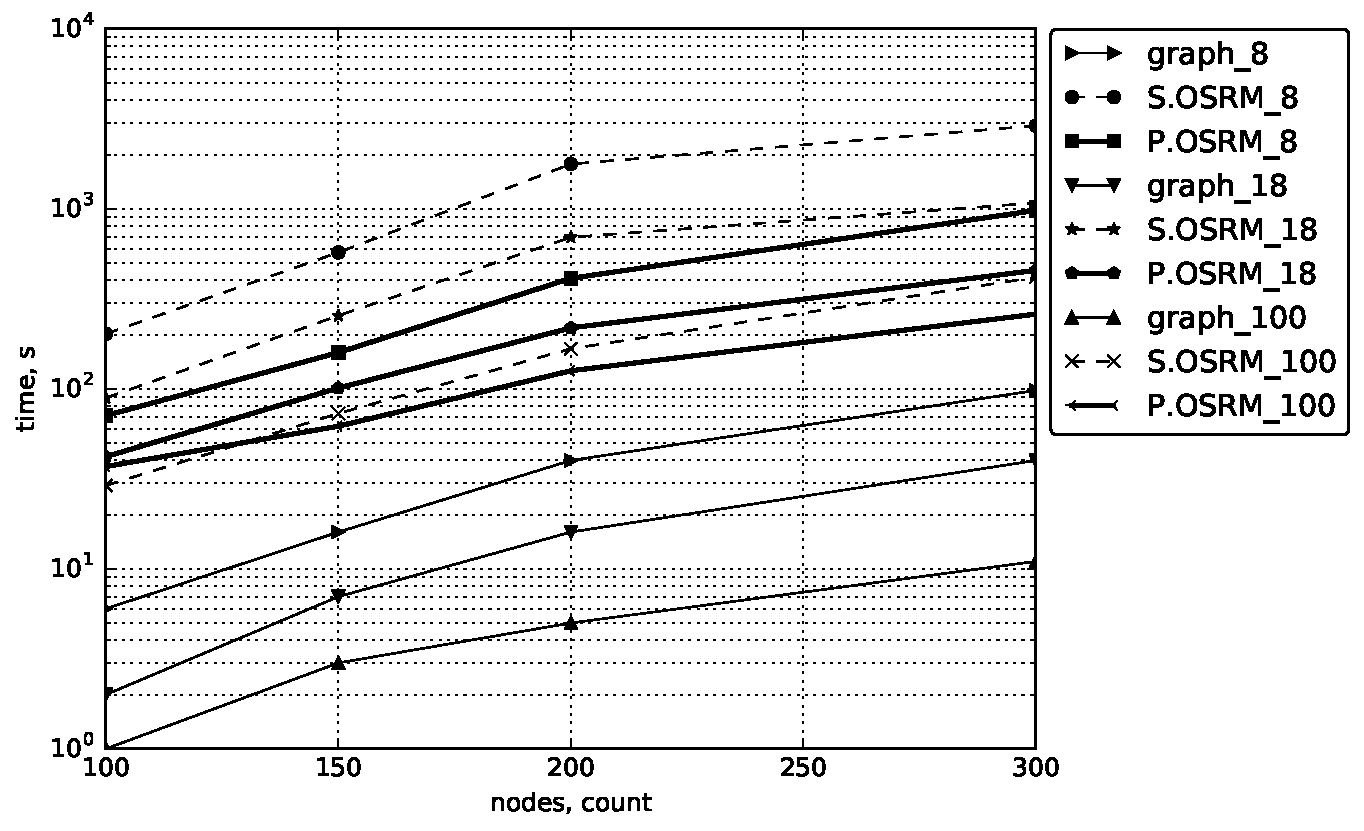
\includegraphics[width=\textwidth]{result-02}
    \caption{Зависимость времени построения от кластеров}
    \label{fig:result-02}
\end{figure}

\begin{figure}[ht!]
    \centering
    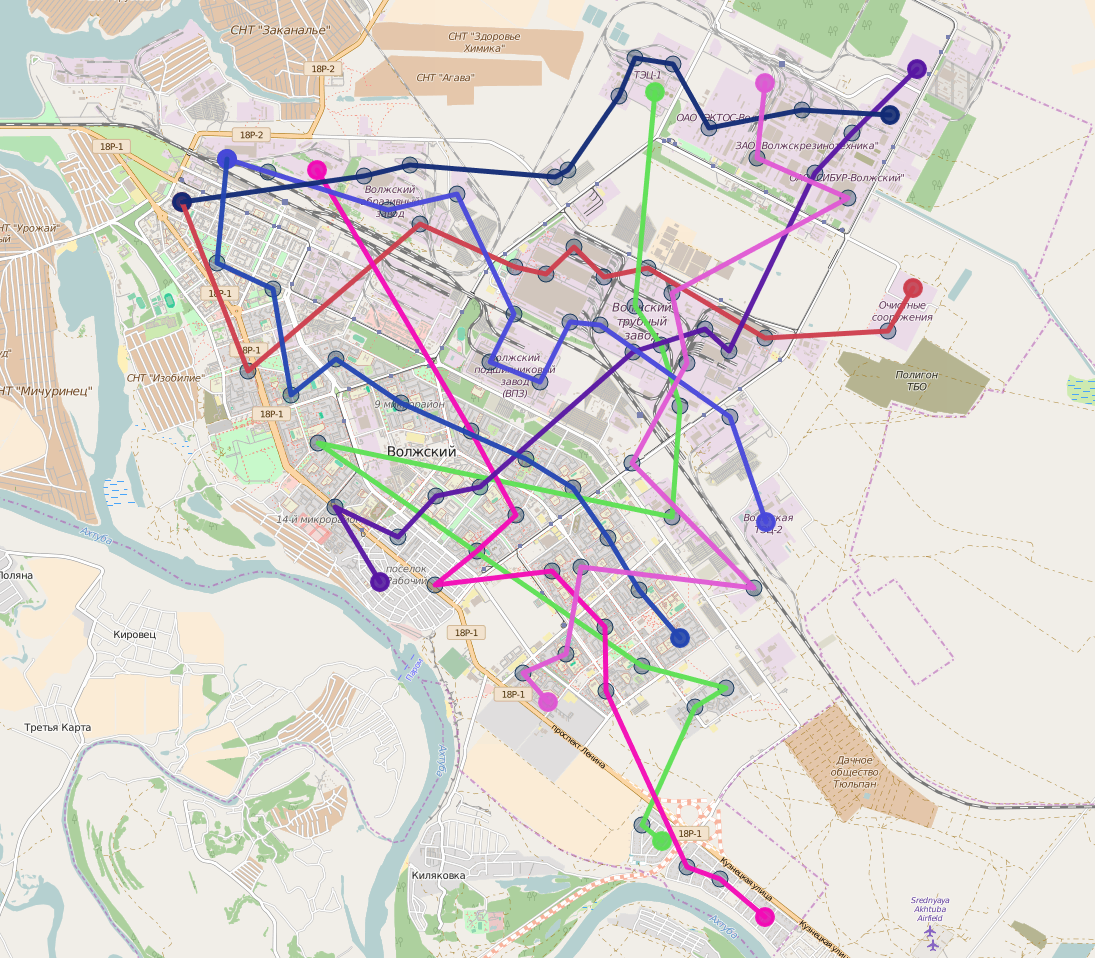
\includegraphics[width=0.8\textwidth]{minimal-01}
    \caption{Использование метрики graph для 100 кластеров и 8 маршрутов.}
    \label{fig:network-01}
\end{figure}

\begin{figure}[ht!]
    \centering
    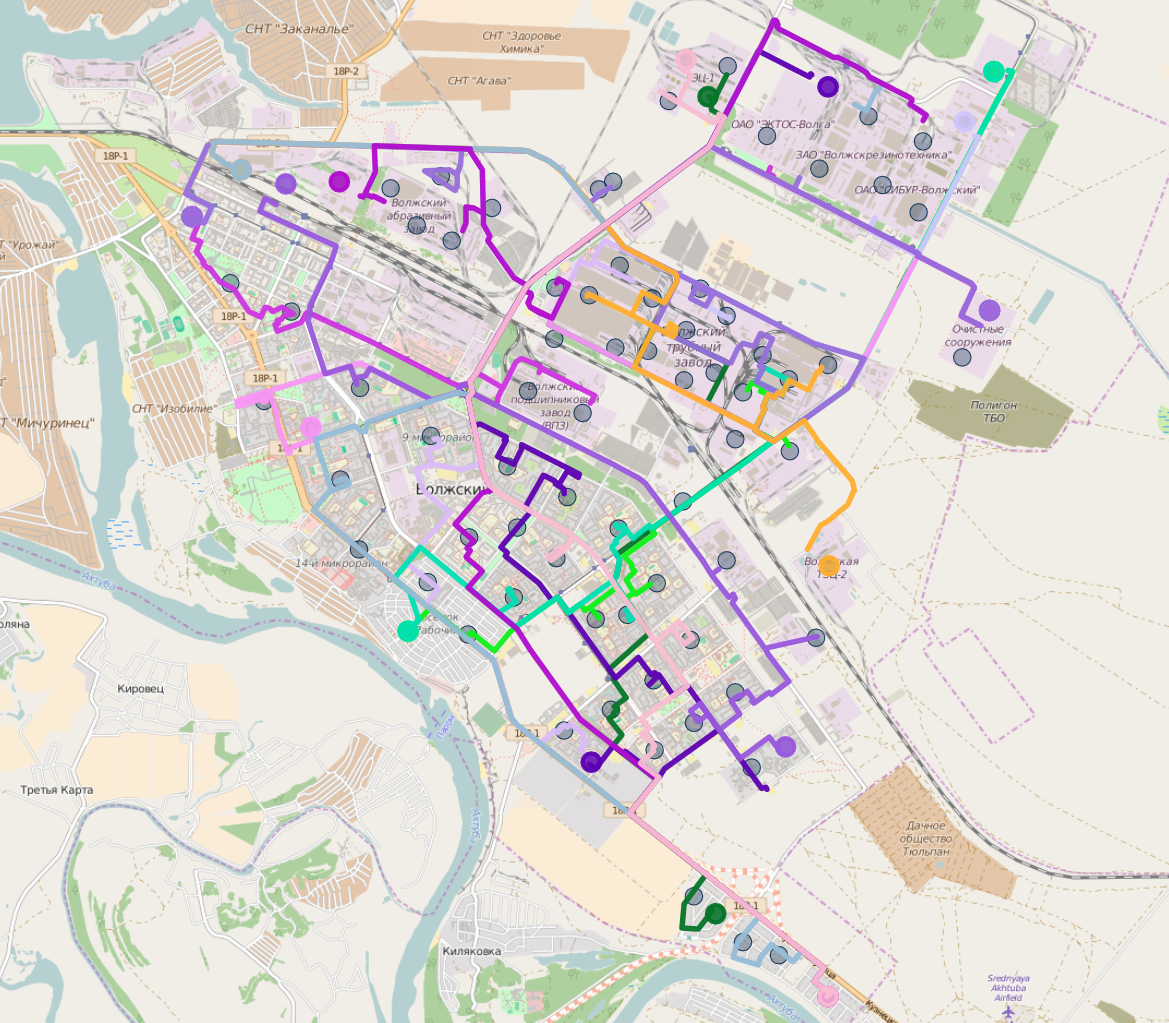
\includegraphics[width=0.8\textwidth]{minimal-02}
    \caption{Использование метрики OSRM для 100 кластеров и 14 маршрутов.}
    \label{fig:network-02}
\end{figure}

\clearpage

\begin{table}[ht!]
    \centering
    \caption{Результаты эксперимента алгоритма из пункта \ref{sec:second_alg}.\\
        Данные представлены в формате минуты:секунды.}
    \label{tab:second_alg}
    \small
    \begin{tabular}{|c|l|c|c|c|c|c|c|l|l|l|c|}
        \hline
        \multicolumn{1}{|l|}{}      &          & \multicolumn{10}{c|}{routes}                                                                                                       \\ \hline
        \multicolumn{1}{|l|}{nodes} & strategy & 8     & 10    & 12    & 14    & 16    & 18    & \multicolumn{1}{c|}{40} & \multicolumn{1}{c|}{60} & \multicolumn{1}{c|}{80} & 100  \\ \hline
        \multirow{3}{*}{100}        & graph    & 0:06  & 0:04  & 0:03  & 0:03  & 0:02  & 0:02  & 0:01                    & 0:01                    & 0:01                    & 0:01 \\ \cline{2-12} 
        & S. OSRM  & 3:22  & 2:35  & 2:01  & 1:44  & 1:40  & 1:29  & 0:17                    & 0:23                    & 0:25                    & 0:29 \\ \cline{2-12} 
        & P. OSRM  & 1:11  & 1:03  & 0:51  & 0:50  & 0:42  & 0:42  & 0:25                    & 0:17                    & 0:34                    & 0:37 \\ \hline
        \multirow{3}{*}{150}        & graph    & 0:16  & 0:12  & 0:10  & 0:08  & 0:07  & 0:07  & 0:04                    & 0:03                    & 0:02                    & 0:03 \\ \cline{2-12} 
        & S. OSRM  & 9:32  & 7:24  & 6:06  & 5:34  & 4:59  & 4:15  & 1:27                    & 1:06                    & 0:57                    & 1:13 \\ \cline{2-12} 
        & P. OSRM  & 2:39  & 2:17  & 1:58  & 1:56  & 1:42  & 1:41  & 1:06                    & 1:13                    & 0:56                    & 1:02 \\ \hline
        \multirow{3}{*}{200}        & graph    & 0:40  & 0:31  & 0:25  & 0:20  & 0:20  & 0:16  & 0:08                    & 0:06                    & 0:05                    & 0:05 \\ \cline{2-12} 
        & S. OSRM  & 29:33 & 22:45 & 18:36 & 16:43 & 13:53 & 11:35 & 3:18                    & 2:20                    & 2:12                    & 2:47 \\ \cline{2-12} 
        & P. OSRM  & 6:51  & 5:23  & 5:06  & 4:07  & 3:48  & 3:38  & 2:08                    & 1:53                    & 1:49                    & 2:06 \\ \hline
        \multirow{3}{*}{300}        & graph    & 1:38  & 1:16  & 1:02  & 0:51  & 0:46  & 0:40  & 0:20                    & 0:14                    & 0:11                    & 0:11 \\ \cline{2-12} 
        & S. OSRM  & 48:20 & 35:24 & 30:00 & 27:17 & 21:06 & 18:01 & 8:41                    & 6:02                    & 6:21                    & 6:57 \\ \cline{2-12} 
        & P. OSRM  & 16:20 & 12:28 & 10:31 & 9:08  & 8:35  & 7:35  & 4:38                    & 4:19                    & 4:46                    & 4:20 \\ \hline
    \end{tabular}
\end{table}

\clearpage

\section{Обсуждение результатов}
\section{Интеграция}

\section{Заключение}